\chapter{Grundlagen}
In diesem Kapitel wird das Vorgehensmodell erläutert sowie alle Tools, die für die erfolgreiche Abwicklung des Projekts
benötigt werden. Außerdem wird die Konzeption der Fragebögen behandelt.

\section{Vorgehensmodelle}\marginpar{\small\(\rightarrow\) {\tiny SKREPEK}}
Vor der Implementierung des Projekts wurden verschiedene methodische Ansätze für das Projektmanagement untersucht. Das
Projektteam entschied sich schnell für ein agiles Vorgehensmodell, um die Dynamik der Planung und Durchführung des Projekts
zu optimieren. Zu Beginn des Projekts wurde Scrum als bevorzugtes Modell ausgewählt. Im folgenden Abschnitt wird eine
detaillierte Erläuterung des Vorgehensmodells präsentiert, gefolgt von einer Begründung für unsere Wahl.

\subsection{Scrum}
Scrum ist ein agiles Projektmanagement-Framework, dass sich auf die effiziente Entwicklung von Produkten und Software
konzentriert. Es legt besonderen Wert auf Zusammenarbeit, Anpassungsfähigkeit und die kontinuierliche Bereitstellung
funktionsfähiger Produktinkremente innerhalb kurzer Entwicklungszyklen, die als Sprints bezeichnet werden.\footnote{Scrum.org \cite{What is Scrum}}\\

Die zuvor skizzierte Definition bietet einen prägnanten Einblick in das agile Vorgehensmodell Scrum. Die herausragenden Merkmale dieses Modells umfassen:

\begin{itemize}
    \item Definition von drei zentralen Rollen, die im Folgenden näher erläutert werden.
    \item Verwaltung des Product Backlogs, der sämtliche Anforderungen enthält.
    \item Iterative und zeitlich definierte Entwicklung von Produkten.
    \item Förderung der autonomen Arbeitsweise des Teams.
    \item Gewährleistung der Gleichberechtigung aller Teammitglieder.
\end{itemize}

\subsubsection{Die drei Rollen in Scrum}
\subsubsection*{Product Owner}
Der Product Owner ist verantwortlich für die Pflege des Product Backlogs und vertritt dabei die fachliche Auftraggeberseite.
Eine zentrale Aufgabe ist die Priorisierung der Elemente im Product Backlog, um den geschäftlichen Wert des Produkts zu
maximieren und die Möglichkeit für frühe Veröffentlichungen essentieller Funktionalitäten zu schaffen. Der Product Owner
nimmt nach Möglichkeit an den täglichen Scrum-Meetings teil, um Einblicke zu gewinnen. Er steht dem Team für Rückfragen
zur Verfügung, um einen reibungslosen Informationsaustausch zu gewährleisten.\footnote{Scrum.org \cite{What is a Product Owner}}

\subsubsection*{Scrum Master}
Der Scrum Master spielt eine zentrale Rolle im Scrum-Prozess und ist für dessen korrekte Umsetzung verantwortlich. Er
fungiert als Vermittler und Unterstützer, um einen optimalen Arbeitsfortschritt zu erzielen und kontinuierliche Optimierung
sicherzustellen. Ein zentrales Anliegen ist die Beseitigung von Hindernissen, um ein reibungsloses Voranschreiten des Teams
zu gewährleisten. Der Scrum Master sorgt für einen effizienten Informationsfluss zwischen dem Product Owner und dem Team,
moderiert Scrum-Meetings und behält die Aktualität der Scrum-Artefakte wie Product Backlog, Sprint Backlog und Burndown
Charts im Blick. Darüber hinaus obliegt es seiner Verantwortung, das Team vor unbefugten Eingriffen während des Sprints
zu schützen.\footnote{Scrum.org \cite{What is a Scrum Master}}

\subsubsection*{Team}
Das Team besteht idealerweise aus sieben Mitgliedern und setzt sich interdisziplinär aus Entwicklern, Architekten,
Testern und technischen Redakteuren zusammen. Es agiert selbstorganisiert und übernimmt die Verantwortung als eigener
Leiter. Es hat die Befugnis, autonom über die Aufteilung von Anforderungen in Aufgaben zu entscheiden und diese auf die
einzelnen Mitglieder zu verteilen. Dadurch entsteht der Sprint Backlog aus dem aktuellen Teil des Product Backlogs.\footnote{Scrum.org \cite{What is a developer}}

\subsubsection{Scrum Meetings}
Alle Anforderungen an das Produkt werden in sogenannten \textit{User Stories} gesammelt, die vorrangig vom Product Owner
im Product Backlog erstellt werden. Während eines Sprints werden die User Stories abgearbeitet. Die Projektentwicklung
nach Scrum besteht aus fünf zentralen Elementen:

\subsubsection*{Sprint Planning Meeting}
Im Sprint Planning Meeting wird das Ziel des folgenden Sprints definiert. Dabei werden die Anforderungen im Product
Backlog, die in diesem Sprint umgesetzt werden sollen, in einzelne Aufgaben zerlegt und anschließend im Sprint Backlog
gesammelt.\footnote{Scrum.org \cite{What is Sprint Planning}}

\subsubsection*{Sprint}
Ein Sprint ist eine Entwicklungsphase, in der eine voll funktionsfähige und potenziell veröffentlichbare Software
entsteht. Die Dauer eines Sprints beträgt typischerweise zwischen 1 und 4 Wochen und ist für alle Sprints gleich lang.\footnote{Scrum.org \cite{What is a Sprint}}

\subsubsection*{Daily Scrum}
Der Daily Scrum ist ein kurzes tägliches Teammeeting im Scrum-Framework. Es dient dazu, den Fortschritt des Teams zu
synchronisieren und potenzielle Hindernisse frühzeitig zu identifizieren. Während dieses Meetings informieren die
Teammitglieder die anderen über den Abschluss ihrer Aufgaben seit dem letzten Treffen, diskutieren, woran sie bis zum
nächsten Treffen arbeiten werden, und geben Einblicke in eventuelle aktuelle Probleme oder Herausforderungen. Dieses
regelmäßige Treffen stellt sicher, dass alle Teammitglieder stets auf dem aktuellen Stand sind. Es fördert eine effektive
Zusammenarbeit und ermöglicht eine zeitnahe Lösung aufkommender Probleme. \footnote{Scrum.org \cite{What is a Daily Scrum}}

\subsubsection*{Sprint Review}
Während des Meetings präsentiert das Entwicklungsteam den Stakeholdern die im Sprint abgeschlossenen Arbeitsergebnisse,
wie zum Beispiel fertige Produktinkremente. Zu den Stakeholdern gehören typischerweise Produktbesitzer, Kunden,
Führungskräfte und andere relevante Interessengruppen.\footnote{Scrum.org \cite{What is a Sprint Review}}

\subsubsection*{Sprint Retrospektive}
Die Sprint Retrospektive ermöglicht es dem Scrum-Team, bestehend aus dem Entwicklungsteam, dem Scrum Master und dem Product
Owner, gemeinsam den abgeschlossenen Sprint zu reflektieren und Möglichkeiten zur kontinuierlichen Verbesserung der Projekteinheit zu
identifizieren.\footnote{Scrum.org \cite{What is a Sprint Retrospective}}
\\

Durch die Elemente des agilen Ansatzes, insbesondere die iterative Natur von Scrum, kann ein optimaler Projektablauf
gewährleistet werden. Die kontinuierliche Zusammenarbeit mit dem Kunden ermöglicht es, Anforderungen und Erwartungen
während des gesamten Entwicklungsprozesses anzupassen und zu verfeinern. Dies führt zu höherer Kundenzufriedenheit und
einem Produkt, das besser den tatsächlichen Bedürfnissen entspricht.

Darüber hinaus bietet regelmäßige Kommunikation und Transparenz innerhalb des Teams und mit den Stakeholdern die Möglichkeit,
Missverständnisse und Probleme frühzeitig zu erkennen und anzugehen. So kann das Team schnell auf Veränderungen reagieren
und den Kurs des Projekts entsprechend anpassen. Dadurch können potenzielle Risiken minimiert und die Effizienz sowie
die Qualität der Arbeit verbessert werden.

\subsection{Begründung der Auswahl}
Die Applikation \textit{Applied Augmented Reality in Education} besteht aus drei verschiedenen Szenarien. Das Team,
bestehend aus vier Schülern, übernahm jeweils einen Teilbereich oder arbeitete in Subteams an einem dieser Szenarien. Dabei
erhielten sie Unterstützung vom betreuenden Lehrer, der stets für Fragen zur Verfügung stand und häufig beratend tätig war.

Als Vorgehensmodell wählte das Team das agile Modell Scrum. Die Scrum-Richtlinien konnten leicht eingehalten werden, da
sich das Team täglich in der Schule traf und auch außerhalb der Schule privat in Kontakt stand. Diese regelmäßige Kommunikation
ermöglichte es dem Team, Änderungen, Probleme und andere Angelegenheiten leicht zu kommunizieren und zu besprechen.

Am Ende jedes Sprints wurden die erreichten Ergebnisse mit dem Betreuer besprochen und Neuerungen vorgestellt. Im Rahmen
der Sprintreviews wurden Feedback zu den Ergebnissen gesammelt und neue Ansichten sowie Denkweisen vom Betreuer eingebracht
und integriert.

Die Sprint Retrospektive ermöglichte den Schülern, einen größeren Mehrwert aus der Projektentwicklung zu ziehen, da sie
neben der Anwendung des Scrum-Prozesses auch ihre Fähigkeiten in den einzelnen Bereichen verbessern konnten. Hierbei
diskutierten und reflektierten sie positive und negative Aspekte.

\section{Projektmanagement-Tools}
Um einen positiven Verlauf des Projekts zu ermöglichen, benötigt man unterstützende
Tools für das Projektmanagement sowie die Verwaltung von Sourcecode.

\subsection{GitHub}
Als Repository für die Source Code Dateien wurde Git in Verbindung mit seiner Webanwendung verwendet. Bei Projektbeginn
galt es, die Entscheidung zu treffen, welche Technologie und welcher Anbieter für das Versionskontrollsystem am besten
geeignet waren.
Andere namhafte Anbieter solcher Plattformen für Verwaltungssysteme sind:
\begin{itemize}
    \item GitLab
    \item SourceForge
    \item BitBucket
\end{itemize}

Die Wahl von GitHub war durch mehrere Aspekte begründet. Zum einen stellt GitHub eine kostenfreie Lösung dar, die es
ermöglicht, ein privates Projekt mit mehreren Mitgliedern ohne Kosten anzulegen. Im Gegensatz dazu bieten einige Plattformen
lediglich eine begrenzte Anzahl von Mitgliedschaften in kostenfreien Projekten an. Die Registrierung erforderte lediglich
einen Account.

Darüber hinaus zeichnet sich GitHub durch eine benutzerfreundliche Oberfläche, eine breite Unterstützung für verschiedene
Programmiersprachen und eine aktive Entwicklergemeinschaft aus. Dies erleichtert die Zusammenarbeit und den Informationsaustausch
im Projektteam.

\subsection{Jira}
Jira wurde als Verwaltungstool für die Vorgänge im Projekt in Verbindung mit seiner Webanwendung verwendet. Auch hier
stand zu Projektbeginn die Frage im Raum, welche Technologie und welcher Anbieter für das Aufgabenmanagement am besten
geeignet waren.
Neben Jira existieren noch weitere namhafte Anbieter solcher Tools wie beispielsweise:
\begin{itemize}
    \item VivifyScrum\footnote{VivifyScrum-Website \cite{https://app.vivifyscrum.com}}
    \item Trelle\footnote{Trello-Website \cite{https://Trello.com}}
\end{itemize}

Die Entscheidung für Jira basierte auf mehreren Überlegungen. Zum einen bietet Jira eine kostenfreie Lösung, die es
ermöglicht, ein SCRUM Board mit mehreren Mitgliedern kostenfrei anzulegen. Ein weiterer entscheidender Faktor war die
direkte Verbindung zu dem GitHub-Repository und die Möglichkeit, neue Branches und Commits direkt in Jira zu erstellen.

Darüber hinaus bietet Jira eine umfassende Funktionalität für das Projektmanagement, einschließlich der Verfolgung von
Aufgaben, der Planung von Sprints und der Erstellung von Berichten. Diese Features ermöglichen es dem Projektteam, den
Fortschritt genau zu überwachen und eventuelle Herausforderungen frühzeitig zu identifizieren und anzugehen.

\section{Fragebögen}\marginpar{\small\(\rightarrow\) {\tiny SKREPEK}}
Um die erstellte Applikation anhand von User-Feedback zu verbessern wurde in dieser Diplomarbeit ein Fragebogen erstellt
und eine Umfrage durchgeführt.

\subsection{Konzeption von Fragebögen}
Bei jeder Umfrage werden Informationen von Personen oder Personengruppen zu der allgemeinen
Umsetzung und dem Verständis der Applikation gesammelt. Diese werden im Anschluss ausgewertet und
interpretiert. Wichtig ist hier den Zweck jeder Umfrage genau zu definieren. Durch präzise und
detailierte Zielsetzungen ist es später dann möglich, den Erfolg der Umfrage zu garantieren.

\subsection{Planung der Fragebogenkonstruktion}
Die sorgfältige Konzeption und Gestaltung eines Fragebogens sind grundlegende Schritte, die bei der Planung einer Erhebung unternommen werden.
Durch eine sorgfältige Planung wird sichergestellt, dass relevante Daten erhoben werden und die spätere Auswertung erleichtert wird.
Aus diesem Grund müssen bereits im Vorfeld verschiedene Entscheidungen getroffen und Definitionen festgelegt werden:

\begin{enumerate}

    \item \textbf{Inhalt}\\
    Die Auswahl der Inhalte ist für die Qualität der erhobenen Daten entscheidend. Es sollte erwogen werden, bestehende
    Fragebögen wiederzuverwenden und gegebenenfalls an die spezifischen Anforderungen der Erhebung anzupassen. Um Missverständnisse
    zu vermeiden, sollten die Fragen klar und prägnant formuliert sein. Die Verwendung validierter Fragebögen kann bei der
    Gewährleistung der Vergleichbarkeit mit anderen Studien hilfreich sein.

    \item \textbf{Umfang}\\
    Ein wichtiger Faktor, der je nach Forschungsziel abgewogen werden muss, ist die Länge des Fragebogens. Das Ziel sollte
    ein ausgewogenes Verhältnis zwischen der Tiefe der Informationen und der Aufrechterhaltung der Teilnahme der Teilnehmer
    sein. Ein zu umfangreicher Fragebogen kann dazu führen, dass die Befragten ermüden und die Qualität der Antworten
    beeinträchtigt wird.

    \item \textbf{Ablauf und zeitlicher Rahmen}\\
    Die Entscheidung bezüglich des Ablaufs und des Zeitrahmens der Befragung beeinflusst die Art der Datensammlung. Die
    Wahl zwischen einer postalischen und einer elektronischen Befragung wirkt sich auf die Antwortzeit und die Effizienz
    der Datenerhebung aus. Bei elektronischen Erhebungen liegen die Ergebnisse oft schneller vor, während bei postalischen
    Erhebungen längere Antwortzeiten möglich sind.

    \item \textbf{Zielgruppe}\\
    Die Definition der Zielgruppe spielt eine wichtige Rolle für die Repräsentativität der Ergebnisse. Die Entscheidung
    für eine Vollerhebung oder eine Stichprobe ist eine Frage der zur Verfügung stehenden Ressourcen und der spezifischen
    Forschungsziele. Eine Vollerhebung kann eine umfangreiche Datenbasis liefern, während eine Stichprobenerhebung
    insbesondere bei großen Zielgruppen effizienter sein kann.

    \item \textbf{Fragetypen und Antwortskalen}\\
    Die Qualität der erhobenen Daten wird durch die Wahl der Art der Fragen und die Wahl der Antwortskalen beeinflusst.
    Geschlossene Fragen mit vorgegebenen Antwortmöglichkeiten erleichtern die quantitative Analyse, während offene Fragen
    die Möglichkeit bieten, qualitative Einsichten zu gewinnen. Die Wahl der Antwortskalen, unabhängig davon, ob es sich
    um Likert-Skalen oder numerische Bewertungen handelt, sollte auf die spezifischen Forschungsziele abgestimmt sein.

    \item \textbf{Ethik und Datenschutz}\\
    Es ist von entscheidender Bedeutung, ethische Aspekte zu berücksichtigen, wie die Anonymität der Teilnehmer zu wahren
    und sensible Informationen zu schützen. Der Fragebogen sollte so konzipiert sein, dass die Integrität der Teilnehmer
    geschützt wird und keine unangebrachten persönlichen Informationen gesammelt werden.

    \item \textbf{Pilotstudie}\\
    Es empfiehlt sich, vor der endgültigen Implementierung des Bogens eine Pilotstudie durchzuführen. Im Rahmen
    dieser Testphase können mögliche Probleme, Unklarheiten oder Missverständnisse bei der Formulierung der Fragen erkannt
    und behoben werden. Das Feedback der Testteilnehmer trägt dazu bei, den Fragebogen noch weiter zu optimieren.
\end{enumerate}
\\

Grundsätzlich werden die \textit{quantitative} und die \textit{qualitative Forschung} unterschieden, wobei Fragebögen zur
\textit{quantitativen Forschung} aufgrund der besseren Vergleichbarkeit leichter zu interpretieren sind.

Bei der Quantifizierung schließt man von der Stichprobe auf die Grundgesamtheit N, wie in Abbildung \ref{fig:GrundgesamtheitStichprobe}
gezeigt. Es ist wichtig, dass die ausgewählte Stichprobe repräsentativ ist. Das bedeutet, dass die Personen, die an der
Stichprobe teilnehmen, die gleichen Voraussetzungen haben wie die Personen, die tatsächlich in der Grundgesamtheit vorkommen.
Es handelt sich hierbei um numerische Daten, die erhoben werden und für die eine Auswertung vorgenommen wird. Von Bedeutung
ist in diesem Zusammenhang das Verhältnis zwischen der untersuchten Stichprobe und der Grundgesamtheit (Population). In
diesem Zusammenhang ist das Verhältnis zwischen der untersuchten Auswahl und der Population von Bedeutung. Alle Merkmale
der Personen in der Auswahl müssen mit den Merkmalen der Personen in der Population übereinstimmen, zum Beispiel Alter
und Geschlecht.\footnote{Vgl. Mayer, \cite{Interview und schriftliche Befragung}, S. 57 ff.}

%Hier Bild für den Zusammenhand
\begin{figure}[H]
    \centering
    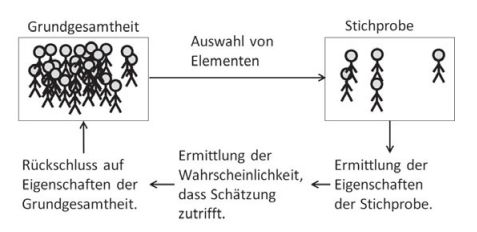
\includegraphics[width=0.8\textwidth]{images/zsmhGrundStich}
    \caption{Zusammenhang zwischen der \textit{Grundgesameheit} und \textit{Stichprobe}\protect\footnotemark}
    \label{fig:GrundgesamtheitStichprobe}
\end{figure}

\footnotetext{Vgl. Brell, \cite{Statistik von Null auf Hundert}, S. 122}


Die qualitative Forschung ist eine Methode zur Auswertung von Daten, die ausschließlich über Sprache (verbal) übermittelt
werden. Diese Methode eignet sich vor allem zur näheren Beschreibung und Analyse von subjektiven Wahrnehmungen, persönlichen
Einstellungen, Motiven und Meinungen der Befragten.\footnote{Vgl. Mayer, \cite{Interview und schriftliche Befragung}, S. 36}

Am sinnvollsten ist eine Kombination von \textit{qualitativen und quantitativen Ergebnissen}. Nach einer quantitativen
Befragung sollte eine stichprobenartige qualitative Befragung durchgeführt werden, um die Ergebnisse besser interpretieren zu können.

Unabhängig davon, ob es sich um qualitative oder quantitative Forschung handelt, sind die drei Gütekriterien \textit{Objektivität,
Zuverlässigkeit und Validität} zu erfüllen.

Sie dienen, den Forschungsprozess zu steuern und zu kontrollieren. Die Validität ist ein Maß für die Brauchbarkeit der
Methode und bezieht sich auf die tatsächliche Fähigkeit zur Messung des gewünschten Wertes. Das Ergebnis ist umso zuverlässiger,
je klarer die Fragen formuliert sind. Entscheidend für die Validität der Analyse ist die Objektivität der Messung. Dabei
ist sowohl die Durchführungsobjektivität des Befragers als auch die Auswertungs- und Interpretationsobjektivität des
Analytikers zu beachten.\footnote{Vgl. Mayer, \cite{Interview und schriftliche Befragung}, S. 54 ff., S. 88.}

Die drei Gütekriterien stehen in einem wechselseitigen Zusammenhang. Nur, wenn die Objektivität gegeben ist, kann die
Reliabilität (Zuverlässigkeit) gewährleistet werden. Ist die Reliabilität gering, kann die Validität nur mit einer gewissen Unsicherheit
vorhergesagt werden.\footnote{Vgl. Bühner, \cite{Einfuehrung in die Test- und Fragebogenkonstruktion}, S. 33 f.}

\subsection{Formulierung der Fragen}
Um eine erfolgreiche Umfrage effizient durchführen zu können, ist eine sorgfältige Vorbereitung erforderlich. Die
Erkenntnis, dass Umfragen nur bestimmte Aspekte eines Themenbereichs abdecken können, ist von entscheidender Bedeutung.
Aus diesem Grund ist eine sorgfältige und präzise Definition dieser Aspekte erforderlich. Besonderes Augenmerk ist darauf
zu richten, dass die Fragen klar formuliert sind.

Die zentrale Priorität bei der Formulierung der Fragen ist die Verständlichkeit und Eindeutigkeit. Die folgenden
Formulierungsrichtlinien sollten unbedingt beachtet werden:
\begin{itemize}
    \item Verwendung von einfachem Vokabular ohne Verwendung von Fachausdrücken, Fremdwörtern oder Ausdrücken aus anderen Sprachen.
    \item Die Fragen prägnant formulieren.
    \item Belastende Begriffe wie \textit{Ehrlichkeit} vermeiden.
    \item Hypothetische Formulierungen ausschließen.
    \item Fokussierung auf ein bestimmtes Thema für jede einzelne Frage.
    \item Vermeidung von Überforderung durch die Bereitstellung einer angemessenen Menge an Informationen pro Frage.
    \item Doppelte Verneinungen vermeiden.\footnote{Vgl. Mayer, \cite{Interview und schriftliche Befragung}, S. 89.}\\
\end{itemize}

Die genannten Kriterien sind besonders wichtig bei schriftlichen Befragungen. Um sicherzustellen, dass die Ergebnisse nicht
verfälscht werden, darf der Interviewer keine zusätzlichen Fragen stellen oder die bereits gestellten Fragen ändern.

Direkte Fragen sind geeignet, um Fakten und Wünsche zu ermitteln, während formulierte Aussagen oder Feststellungen eher
dazu dienen, die Bewertung durch die Befragten in Erfahrung zu bringen. Diese Techniken werden hauptsächlich zur Erfassung
von Einstellungen, Wahrnehmungen und Meinungen eingesetzt.

\subsection{Arten von Fragen}
In Abhängigkeit von den Anforderungen der jeweiligen Evaluation können sowohl offene als auch geschlossene Fragen gestellt werden.

Bei offenen Fragen handelt es sich um Fragen, bei denen keine Antwortmöglichkeiten vorgegeben werden. Im Anschluss an die
Frage sollte ausreichend Platz für die Beantwortung der Frage gelassen werden. Dieser Fragetyp sollte in den folgenden
Fällen verwendet werden:
\begin{itemize}
    \item Wenn die Anzahl der Antwortmöglichkeiten unbekannt ist.
    \item Wenn die Formulierung der Antwort des Auskunftspflichtigen für die Auswertung von Bedeutung ist.
    \item Wenn das Ziel der Erhebung darin besteht, die Unwissenheit und Meinung zu ermitteln.\\
\end{itemize}

Im Gegensatz zu offenen Fragen gibt es bei geschlossenen Fragen vordefinierte Antwortmöglichkeiten. Die Teilnehmerinnen
und Teilnehmer wählen ihre Antworten aus einer vorgegebenen Liste aus oder entscheiden sich zwischen den vorgegebenen
Optionen. Es gibt verschiedene Szenarien, in denen der Einsatz von geschlossenen Fragen sinnvoll ist:

\begin{itemize}
    \item Wenn die Anzahl der möglichen Antwortalternativen begrenzt und bekannt ist.
    \item Bei Umfragen, die quantitative Daten für eine statistische Auswertung erfordern.
    \item Wenn die Standardisierung der Antworten wichtig ist, um eine konsistente Analyse zu ermöglichen.\footnote{Vgl. Scholl, \cite{Die Befragung}, S. 157.}
\end{itemize}

In Bezug auf die geschlossenen Fragen ist es noch wichtig anzumerken, dass es im Wesentlichen drei Möglichkeiten für die
Benennung oder Kennzeichnung gibt:
\begin{enumerate}
    \item \textbf{Numerische Benennung}\\
    Die numerische Benennung ist ein klassisches Notationssystem mit semantischer Bedeutung. Jede Note oder Zahl ist
    eindeutig einer sprachlichen Formulierung zugeordnet. Der Abstand zwischen den einzelnen Noten ist dabei gleich groß.
    \item \textbf{Kennzeichnung durch Formen}\\
    Eine Möglichkeit, geschlossene Fragen zu kennzeichnen, besteht darin, bestimmte Formen wie Kreise, Kästchen oder
    grafische Skalen (Symbole) zu verwenden.
    \item \textbf{Sprachliche Benennung}\\
    Die Benennung von geschlossenen Fragen erfolgt durch klare sprachliche Ausdrücke oder Texte, welche die verschiedenen
    Antwortoptionen definieren.\footnote{Vgl. Scholl, \cite{Die Befragung}, S. 164 ff.}
\end{enumerate}

\subsection{Struktur und Gliederung von Fragebögen}
Die Struktur und Gliederung eines Fragebogens spielen eine entscheidende Rolle bei der Erhebung von Daten. Ein gut
durchdachter Aufbau gewährleistet nicht nur eine klare und präzise Erfassung der benötigten Informationen, sondern
erleichtert auch die Analyse der Ergebnisse. Bei der Gestaltung eines Fragebogens sollten mehrere wichtige \textit{Schlüsselelemente}
berücksichtigt werden.

\textit{Fragetypen} sind ein zentraler Aspekt bei der Strukturierung von Fragebögen. Die geschickte Kombination von
\textit{geschlossenen} und \textit{offenen} Fragen ermöglicht es, eine umfassende Datenerhebung durchzuführen und einen
tieferen Einblick zu gewinnen.

Die \textit{Reihenfolge} der Fragen sollte einer sinnvollen \textit{Sequenz} und \textit{Logik} folgen. Der Fragebogen
sollte mit allgemeinen und weniger sensiblen Fragen beginnen, um das Vertrauen der Teilnehmer zu gewinnen. Danach sollten
spezifischere und möglicherweise persönlichere Fragen gestellt werden.

\textit{Klarheit} ist entscheidend. Klare Anweisungen, eine gut lesbare Schrift und genügend Leerraum tragen dazu bei,
Missverständnisse zu vermeiden. Sie ermutigen die Teilnehmer, präzise Antworten zu geben.

Vor dem endgültigen Einsatz des Fragebogens empfiehlt sich die Erprobung des Fragebogens im Rahmen von \textit{Pilotstudien}.
Dadurch können mögliche Probleme in Bezug auf \textit{Verständlichkeit}, \textit{Länge} und \textit{Schwierigkeitsgrad}
der Fragen identifiziert werden, bevor der endgültige Fragebogen an die Zielgruppe verteilt wird.

Die Beachtung dieser Grundsätze bei der Strukturierung und Gliederung von Fragebögen trägt dazu bei, zuverlässige und
aussagekräftige Daten für die Analyse zu gewinnen.

\subsection{Mögliche Verfälschung des Resultats}
Die Zuverlässigkeit von Umfrageergebnissen kann durch verschiedene Arten der Verfälschung beeinträchtigt werden. Zwei
häufige Verfälschungsarten sind:
\begin{itemize}
    \item \textbf{Simulation}: Teilnehmer neigen dazu, ihre Antworten absichtlich zu verfälschen, um ein bestimmtes Bild
    von sich selbst zu vermitteln. Dies kann dazu führen, dass die gegebenen Antworten nicht mit den tatsächlichen
    Meinungen oder Verhaltensweisen übereinstimmen und somit zu einer Verfälschung der Daten führen.

    \item \textbf{Dissimulation}: Es handelt sich hierbei um die bewusste Verzerrung von Informationen durch Teilnehmer
    mit dem Ziel, bestimmte Aspekte zu verschleiern oder zu verheimlichen. Diese Verzerrung kann dazu führen, dass die
    gewonnenen Daten nicht der Realität entsprechen und somit die Verlässlichkeit der Ergebnisse der Erhebung in Frage
    gestellt wird.\footnote{Vgl. Bühner, \cite{Einfuehrung in die TEst und Fragebogenkonstruktion}, S. 56.}\\
\end{itemize}

Eine Vielzahl von Faktoren kann Verfälschungen auslösen. Gesellschaftliche Normen üben oft Druck auf den Einzelnen aus,
sich selbst in einem positiven Licht darzustellen, was zu einem Verhalten führen kann, das eine Simulation darstellt. Auf
der anderen Seite kann die Furcht vor sozialen Konsequenzen oder persönlichen Nachteilen dazu führen, dass Individuen
Aspekte ihrer selbst zurückhalten oder verbergen.\footnote{Vgl. Bühner, \cite{Einfuehrung in die TEst und Fragebogenkonstruktion}, S. 59.}

Ein umfassendes Verständnis der Ursachen von Simulation und Dissimulation ist entscheidend für die Entwicklung wirksamer
Strategien, mit denen diese Verfälschungen in der Umfrageforschung minimiert werden können.

\subsection{Auswertung von Fragebögen}
Die Hauptintention einer Fragebogenerhebung besteht darin, eine homogene Vergleichbarkeit der individuellen Antworten der
Befragten zu gewährleisten. Dies ermöglicht eine fundierte statistische Auswertung. Eine unabdingbare Voraussetzung, um
aus den erhobenen Fragebogendaten inhaltlich sinnvolle Aussagen ableiten zu können, ist die Umrechnung der qualitativen
Antworten in quantitative Werte. Diese Umrechnung erfolgt insbesondere bei computergestützten Verfahren automatisch.

Offene Fragen erfordern eine inhaltliche Auswertung, die in der Regel in Form einer Häufigkeitsanalyse erfolgt, bei der
ähnliche Antworten zu Kategorien zusammengefasst werden. Auf diese Weise ist es möglich, die Anzahl der Befragten zu
ermitteln, die eine vergleichbare Aussage getroffen haben.

Die Auswertung geschlossener Fragen ist im Allgemeinen mit geringerem Aufwand verbunden, da die Antwortmöglichkeiten
bereits vorgegeben sind und jede einzelne Antwort zu einer dieser vorgegebenen Möglichkeiten passen muss.

Für eine angemessene grafische Darstellung der analysierten Daten sind Kreis-, Balken- und Säulendiagramme besonders
geeignet. Während Balken- und Säulendiagramme die absoluten Häufigkeiten der Antworten visualisieren und damit Unterschiede
in der Anzahl der Antworten deutlich machen, eignen sich Kreisdiagramme besonders, um relative Häufigkeiten, ausgedrückt
in Prozent, darzustellen.

\subsection{Planung und Erstellung eines Fragebogens}
Im Verlauf dieser Diplomarbeit wurde ein Fragebogen gemäß den erläuterten Regeln und Grundlagen entwickelt. Der Fragebogen
soll am \textit{Tag der offenen Tür} an der HTBLuVA Wiener Neustadt in der Abteilung Informatik am 01.12.2024 durchgeführt
werden. In der Planungsphase wurde das allgemeine Layout des Fragebogens festgelegt. Anschließend wurden im Projektteam
Fragen zusammengestellt, die zur Weiterentwicklung der Applikation beitragen sollen. Der Fragebogen wurde mithilfe der
Markup-Sprache \textit{LaTeX} erstellt.

\subsection{Struktur und verwendete Fragetypen}
Eine klare und logische Struktur des Fragebogens sowie die Auswahl geeigneter Fragetypen spielen eine entscheidende Rolle,
um es dem Befragten zu erleichtern, die Fragen zu beantworten, und seine Motivation aufrechtzuerhalten. Der Fragebogen
beginnt mit einer kurzen Einleitung und Begrüßung, um dem Befragten den Zweck des Fragebogens und den Grund für seine
Durchführung zu vermitteln.

Bei der Auswahl der Fragetypen wurde bewusst entschieden, ausschließlich geschlossene Fragen zu verwenden. Diese Entscheidung
basierte auf zwei Hauptüberlegungen. Erstens sollte die begrenzte Zeit am Tag der offenen Tür effizient genutzt werden,
und es galt, die Besucher nicht zu lange aufzuhalten. Daher wurde es als taktisch sinnvoll erachtet, keine offenen Fragen
einzubeziehen. Zweitens erleichtern geschlossene Fragen dem Projektteam die Umwandlung quantitativer Befragungsergebnisse
in qualitative Werte. Außerdem ermöglichte diese Entscheidung dem Projektteam, spezifische Bereiche einzugrenzen, in denen
bereits bekannt war, dass Verbesserungsbedarf besteht.

\subsection{Pilotstudio des Fragebogens}
Um Missverständnisse oder Unklarheiten bezüglich der gestellten Fragen zu vermeiden, wurde vor der endgültigen Durchführung
der Befragung ein Pilotversuch in einer Abschlussklasse der HTBLuVA Wiener Neustadt, Abteilung Informatik, durchgeführt.
Die Ergebnisse dieser Pilotstudie zeigten, dass die gestellten Fragen verständlich waren und ohne größere Probleme beantwortet
werden konnten.

\subsection{Auswertung des erstellten Fragebogens}
Um die Ergebnisse detailliert zu präsentieren, wird in diesem Abschnitt ein realer Fragebogen verwendet, der während des
\textit{Tags der offenen Tür} der HTBLuVA Wiener Neustadt, Abteilung Informatik eingesetzt wurde. Die Fragen werden zunächst
aufgeführt, gefolgt von einer Analyse der Ergebnisse. Für diese Analyse wird das Tool \textit{Excel} verwendet, um die
\textit{qualitativen} Antworten in \textit{quantitative} Werte umzurechnen.

Diese Vorgehensweise ermöglicht es, die gesammelten Daten konkret zu veranschaulichen und deren Bedeutung für das Entwicklerteam
besser verständlich zu machen.

\begin{quote}
    Während des Tages der offenen Tür im Schuljahr 2023/2024 (25 Personen) und in einer Abschlussklasse 5CHIF 2023 / 24 (14 Personen)
    einer Schule mit Matura wurde eine Umfrage durchgeführt, um die Nutzermeinungen zur aktuellen Anwendung zu erfassen.
    Das Ziel dieser Umfrage bestand darin zu ermitteln, ob die zugrunde liegenden ausgewählten Konzepte der Informatik verstanden wurden und ob
    potenzielle Verbesserungsmöglichkeiten vorliegen.

    Anschließend wurden sieben Personen (Stichprobe) der Abschlussklasse befragt, um potenzielle Verbesserungsvorschläge
    zu ermitteln. Das Ziel dieser Umfragen bestand darin, Personen zu befragen, die bereits über grundlegendes IT-Wissen
    verfügen und dadurch besser beurteilen können, welche Aspekte verbessert werden können.
\end{quote}

Der durchgeführte Fragebogen bestand aus fünf geschlossenen Fragen, wobei bei zwei Fragen die Möglichkeit bestand, mehrere
Antworten auszuwählen. Die Entscheidung, ausschließlich geschlossene Fragen zu verwenden, wurde getroffen, um das Feedback
für das Projektteam leichter auswertbar zu machen und um die Umsetzung von Verbesserungen im Nachhinein durch diese quantitative
Befragung zu erleichtern. Die Fragen samt Antwortmöglichkeiten und die zugehörige Auswertung sind wie folgt:
\begin{itemize}
    \item \textbf{1. Frage:} Wie leicht war es für Sie, dass Prinzip des \textit{Nachrichten Austauschs} zwischen zwei PCs in der Applikation zu verstehen?
    \\
    \\
    \textbf{Antwortmöglichkeiten:} \\
    Sehr schwer(5), Schwer(4), Mittel(3), Leicht(2), Sehr leicht(1)
    \\
    \\
    \textbf{Auswertung:}
    \begin{figure}[H]
        \centering
        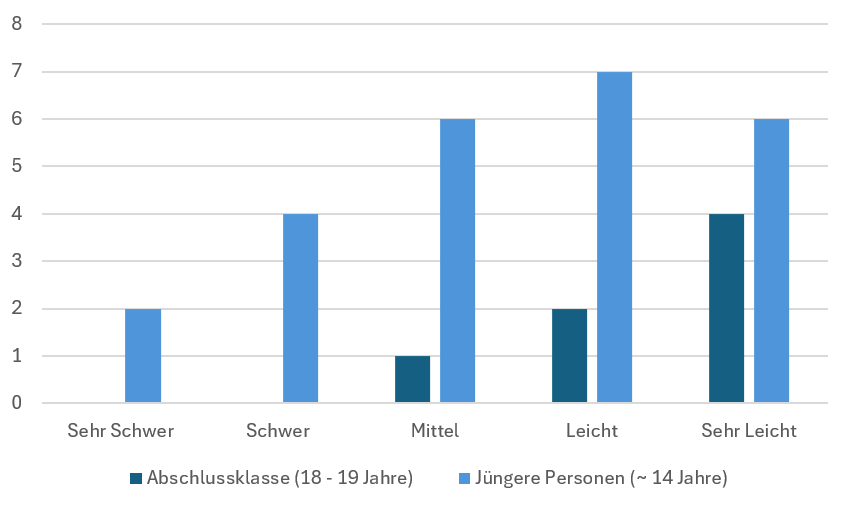
\includegraphics[width=0.7\textwidth]{images/AuswertungFrage1}
        \caption{Auswertung Frage 1}
        \label{fig:fr1}
    \end{figure}
    \\
    \item \textbf{2. Frage:} Konnten Sie das Knapsack-Problem in der Applikation ohne Probleme nachvollziehen?
    \\
    \\
    \textbf{Antwortmöglichkeiten:}\\
    Nein nicht wirklich(3), Ja mit einigen Schwierigkeiten(2), Ja problemlos(1)
    \\
    \\
    \textbf{Auswertung:}
    \begin{figure}[H]
        \centering
        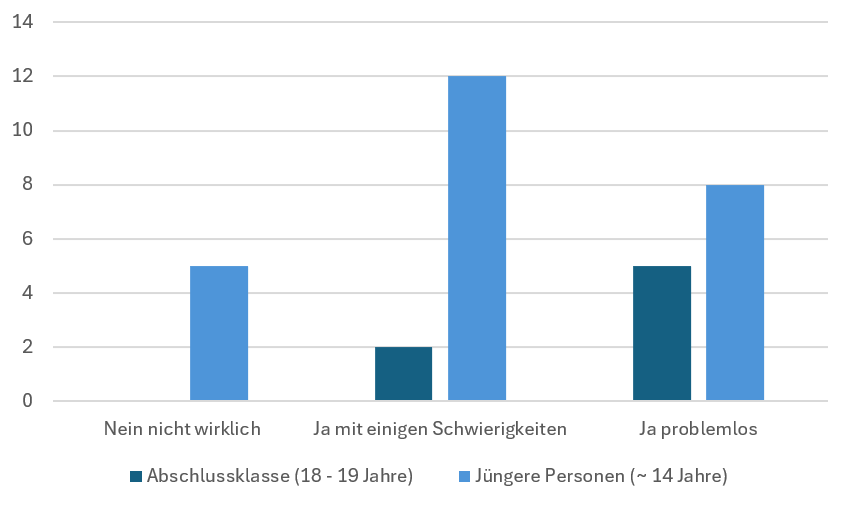
\includegraphics[width=0.7\textwidth]{images/AuswertungFrage2}
        \caption{Ergebnis Frage 2}
        \label{fig:fr1}
    \end{figure}
    \\
    \item \textbf{3. Frage:} Wie sehr hat die AR-Technolgie Ihnen dabei geholfen die Informatik Prinzipien zu verstehen?
    \\
    \\
    \textbf{Antwortmöglichkeiten:}\\
    Sehr negativ(5), Negativ(4), Neutral(3), Positiv(2), Sehr positiv(1)
    \\
    \\
    \textbf{Auswertung:}
    \begin{figure}[H]
        \centering
        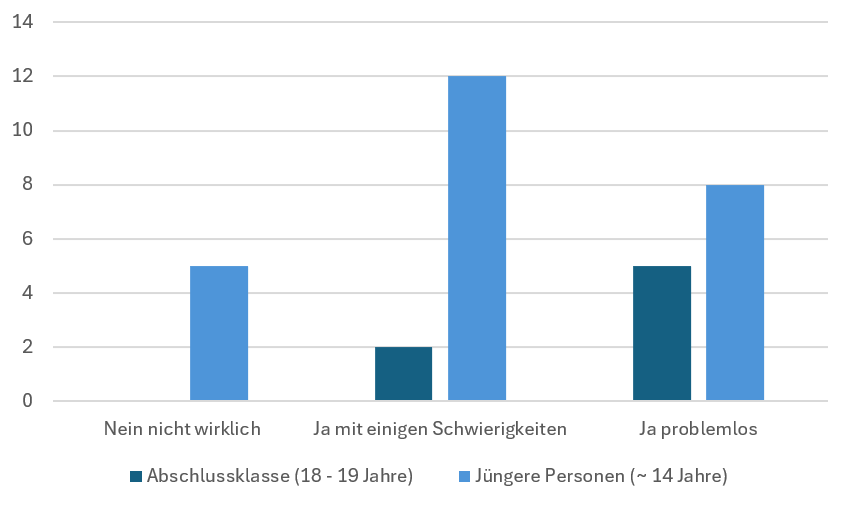
\includegraphics[width=0.7\textwidth]{images/AuswertungFrage2}
        \caption{Ergebnis Frage 3}
        \label{fig:fr1}
    \end{figure}
    \\
    \item \textbf{4. Frage:} Welche der folgenden Aspekte haben Ihnen am meisten gefallen? (Mehr als eine Auswahl möglich)
    \\
    \\
    \textbf{Antwortmöglichkeiten:}\\
    Lernfördernd, Benutzerfreundlichkeit, Kreativität, Innovativ, Interaktiv
    \\
    \\
    \textbf{Auswertung:}
    \begin{figure}[H]
        \centering
        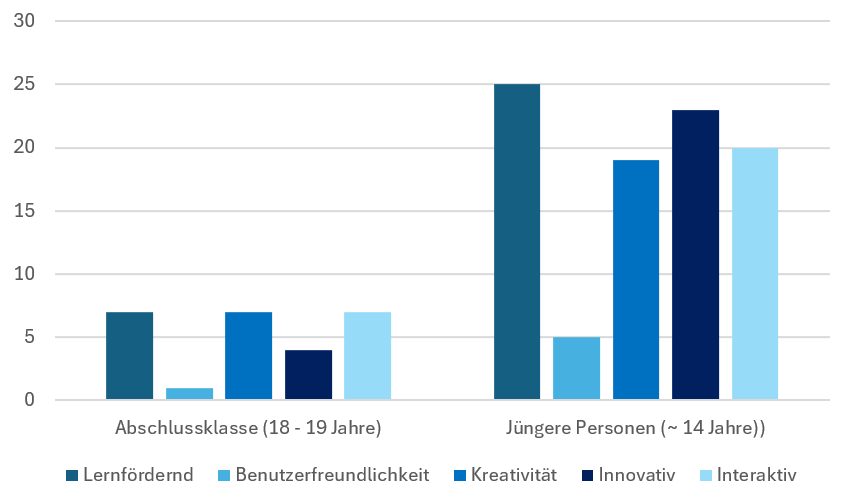
\includegraphics[width=0.7\textwidth]{images/AuswertungFrage4}
        \caption{Ergebnis Frage 4}
        \label{fig:fr1}
    \end{figure}
    \\
    \item \textbf{5. Frage:} Welche der folgenden Aspekte sind noch verbesserungswürdig? (Mehr als eine Auswahl möglich)
    \\
    \\
    \textbf{Antwortmöglichkeiten:}\\
    Tips / Anweisungen, Leistungsfähigkeit, Inhalt, Stabilität, Übersichtlichkeit
    \\
    \\
    \textbf{Auswertung:}
    \begin{figure}[H]
        \centering
        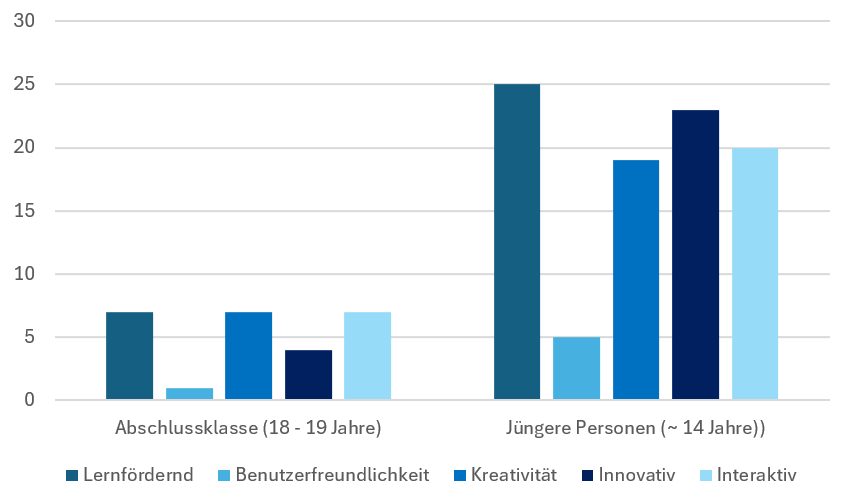
\includegraphics[width=0.7\textwidth]{images/AuswertungFrage4}
        \caption{Ergebnis Frage 5}
        \label{fig:fr1}
    \end{figure}
\end{itemize}

Anhand der Auswertungen des Fragebogens wird deutlich, dass die Antworten der befragten Personen am Tag der offenen Tür
und von den Personen der Abschlussklasse stark voneinander abweichen. Dies wird besonders bei den letzten beiden Fragen,
die sich auf Aspekte, die dem Benutzer gefallen, und Verbesserungsmöglichkeiten beziehen, deutlich. Hier ist nämlich klar
zu erkennen, dass die Personen der Abschlussklasse im Vergleich zu den am Tag der offenen Tür Befragten Person signifikant
mehr Angaben dazu gemacht haben. Dies lässt sich darauf zurückführen, dass sie über deutlich mehr Erfahrung im Bereich
der Entwicklung von Applikationen verfügen und generell ein vertieftes Verständnis der Informatik besitzen. Ein erfreuliches
Ergebnis ist jedoch, dass ein Großteil sowohl der am Tag der offenen Tür befragten als auch der in der Abschlussklasse
befragten Personen die vermittelten Prinzipien der Informatik gut verstanden hat und auch, dass der Einsatz von AR-Technolgie
dabei geholfen hat diese zu verdeutlichen.

Zu erwähnen ist, dass bei der Auswertung insbesondere bei der vorletzten Frage festgestellt wurde, dass die Applikation
als nicht benutzerfreundlich bewertet wurde. Dieses Ergebnis war jedoch erwartet, da zum Zeitpunkt der Befragung das
Projekt noch in einem sehr frühen Entwicklungsstadium war und daher einige essenzielle Funktionen und Erweiterungen wie
Anweisungen und Tipps, Performance und Inhalt fehlten.

Darüber hinaus hat diese Befragung und Auswertung wichtige Ergebnisse geliefert, die dazu beigetragen haben, viele Aspekte
der Applikation maßgeblich zu erweitern und zu verbessern.